\clearpage
\section{Problembeskrivelse}
\label{problemBeskrivelse}


%Her kan du skrive om din problembeskrivelse

I dette designnotatet skal det designes en operasjonsforsterker på transistor nivå. En ideell operasjonsforsterkar har følgene egenskaper og modell som vist i fig \ref{fig:opamp_ideal}.
\begin{itemize}
    \item Inngangsimpedansen til $R_i = \infty$
    \item Utgangsimpedansen til $R_o = 0$
    \item Utgangen er gitt som 
    \begin{equation}
        V_{out} = f(V_+ - V_-) = \begin{cases} 
                                    min \{V, A(v^+ - v^-)\}\ for\ v^+ - v^- > 0 \\
                                    max\{V, A(v^+ - v^-)\}\ for\ v^+ - v^- < 0
                                \end{cases}
    \end{equation}
Spesielt i dette designnotatet skal de følgene egenskapene undersøkest nærmere:
    \begin{itemize}
        \item forsterkningen $A$ ved sinuspåtrykk med frkvens $f = 1kHz$ og 
        \item Total harmonisk distorsjon (THD) ved sinuspåtrykk med frekvens $f = 1kHz$

    \end{itemize}
De to pungtene skal undersøkest med to forskjellige lastmotstander $R_L = 100k\Omega$ og $R_L = 100\Omega$. Det skal også undersøkest hvor godt kretsløsningen virker som en opamp i en inverterende forsterker med forsterkning $A = -10$ og $R_L = 1k\Omega$. Sammenlign dette med ved både åpen løkke forsterkning og negativ tilbakekobling.
\end{itemize}

\begin{figure}[H]
    \centering
    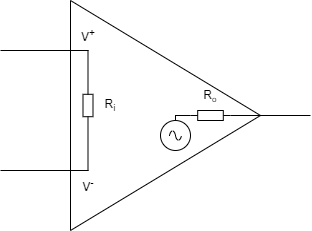
\includegraphics[width=0.4\textwidth]{Bilder/opamp_ideell.drawio.png}
    \caption{Ideell opamp modell}
    \label{fig:opamp_ideal}
\end{figure}